\documentclass{article}
\usepackage{graphicx}

\title{My First Document}
\author{Stefan J. Schmidt}

\begin{document}
\maketitle

\begin{abstract}
Smartphones are increasingly being used to store personal information as well as
to access sensitive data from the Internet and the cloud. Establishment of the
identity of a user requesting information from smartphones is a prerequisite for
secure systems in such scenarios. In the past, keystroke-based user
identification has been successfully deployed on production-level mobile devices
to mitigate the risks associated with naive username/password based
authentication. However, these approaches have two major limitations: they are
not applicable to services where authentication occurs outside the domain of the
mobile device such as web-based services; and they often overly tax the limited
computational capabilities of mobile devices. In this paper, we propose a
protocol for keystroke dynamics analysis which allows web-based applications to
make use of remote attestation and delegated keystroke analysis. The end result
is an efficient keystroke-based user identification mechanism that strengthens
traditional password protected services while mitigating the risks of user
profiling by collaborating malicious web services. We present a prototype
implementation of our protocol using the popular Android operating system for
smartphones.
\end{abstract}

\section{Introduction}
This is going to be a normal paragraph.

\subsection{Some Background}
And some more text here.

\subsubsection{Drilled Down}\label{sec:drilled-down}
Even more text.

\newpage

\section{More Stuff}
Insert a figure in the section.

\begin{figure}
\centering
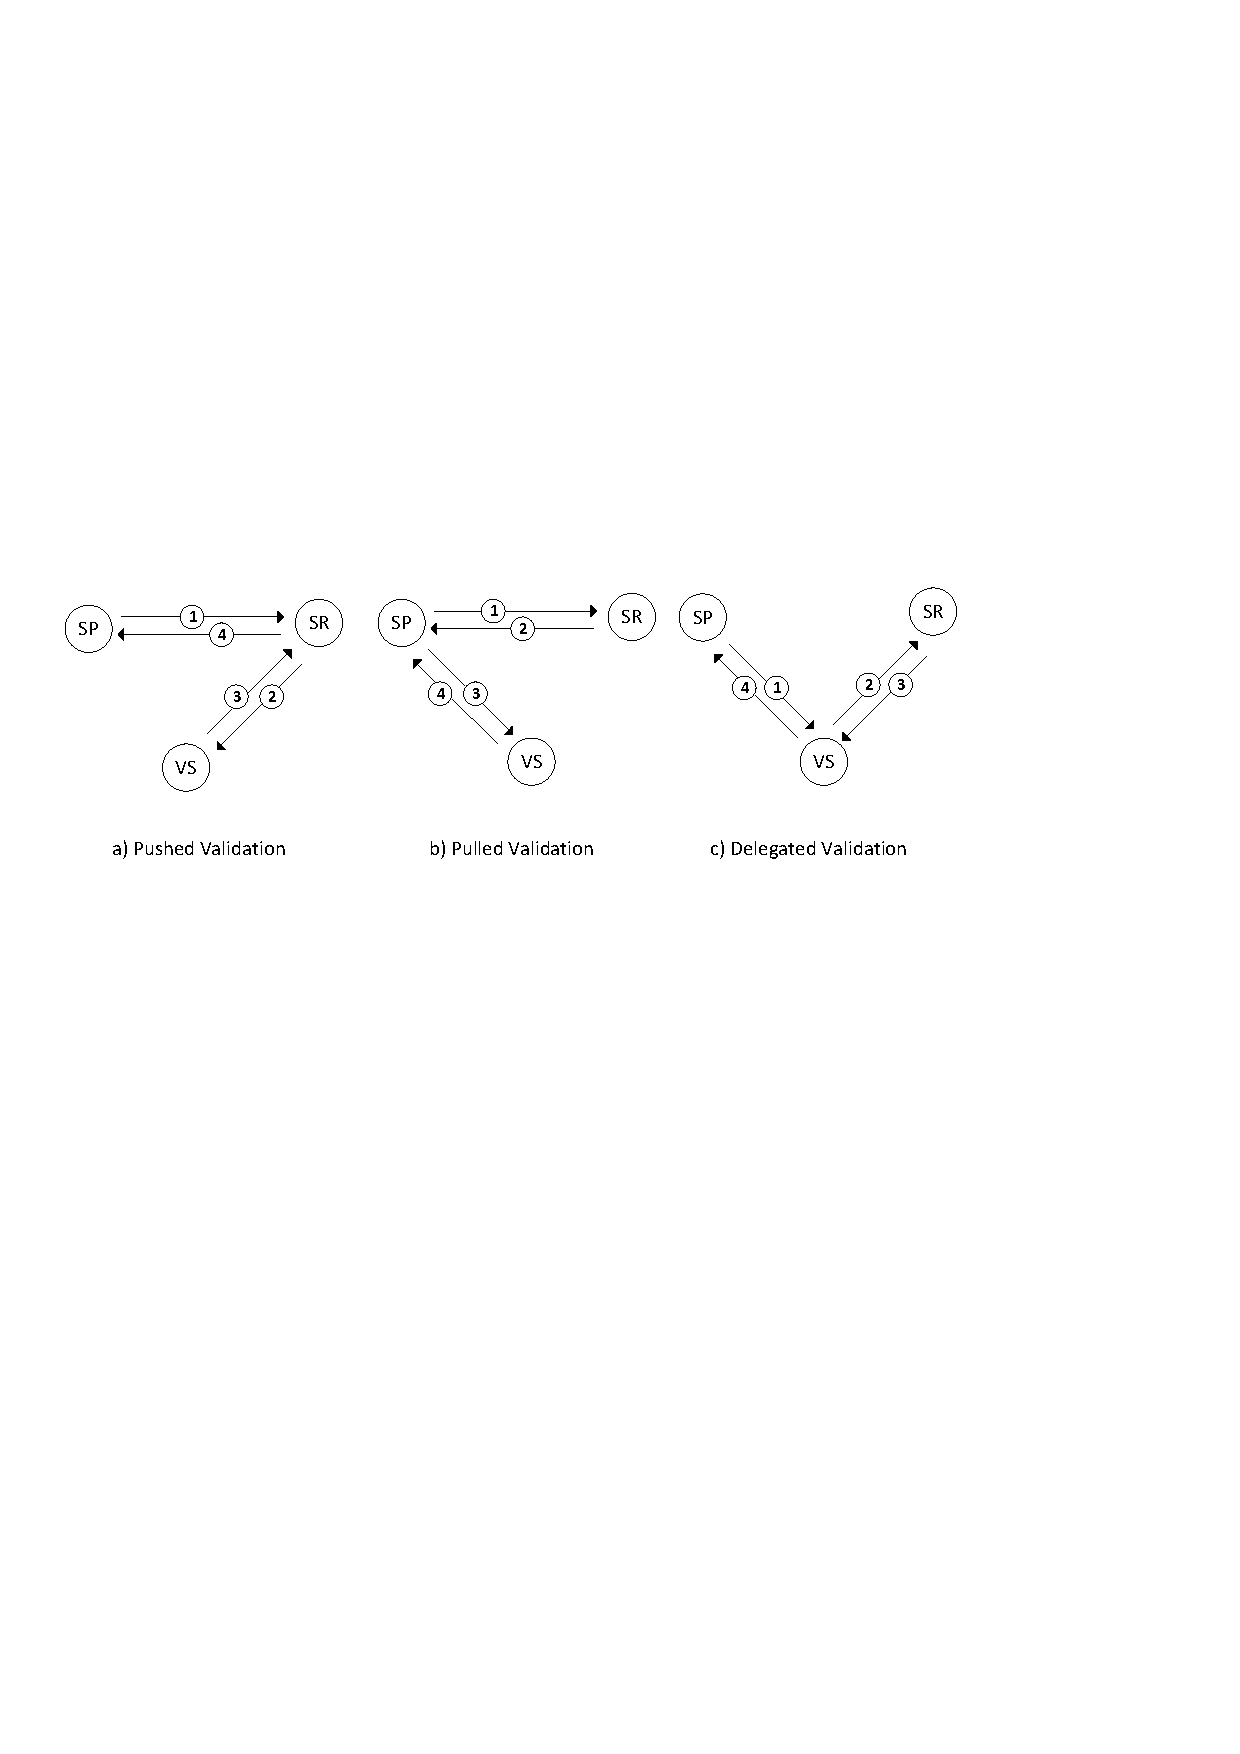
\includegraphics[width=0.5\textwidth]{att-models-base}
\caption{My First Figure}\label{fig:first-figure}
\end{figure}

\begin{figure}
\centering
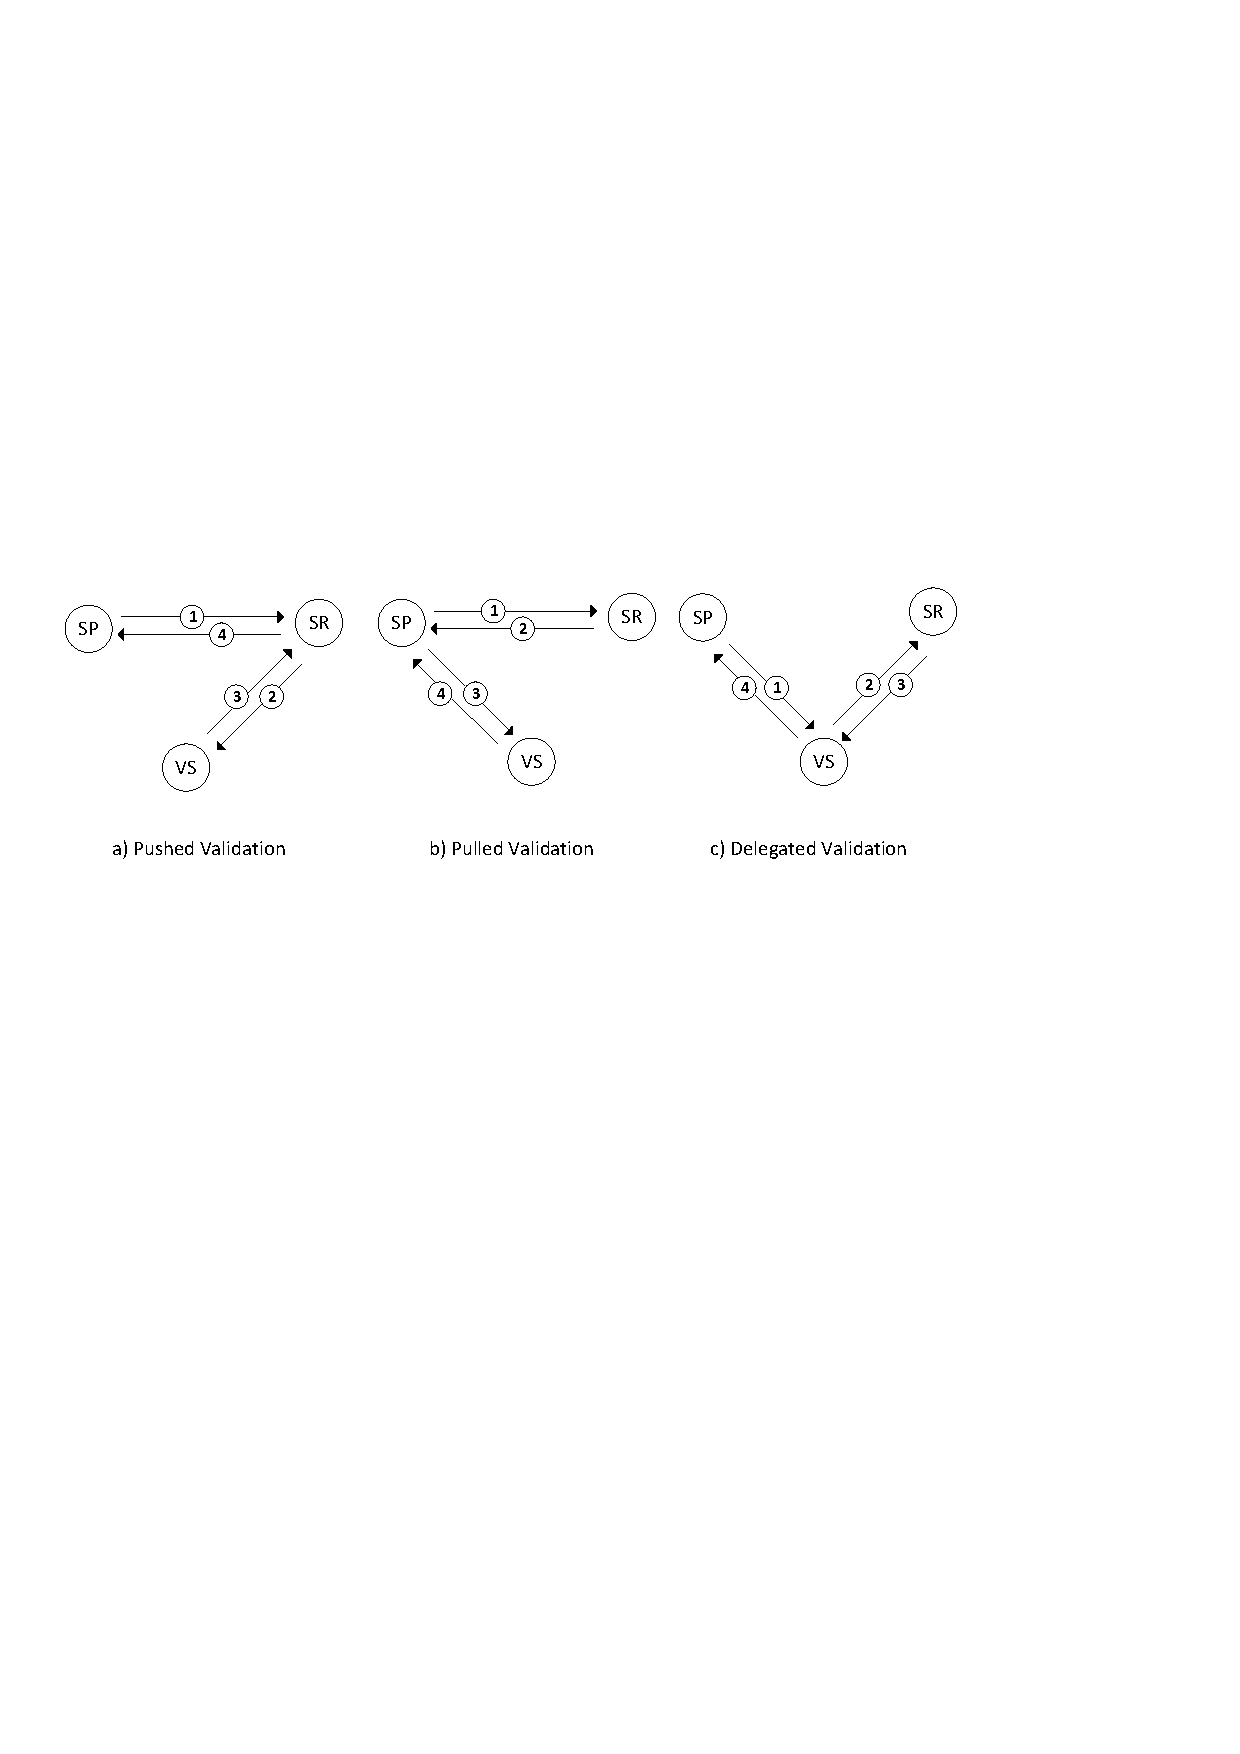
\includegraphics[width=0.5\textwidth]{att-models-base}
\caption{My Second Figure}\label{fig:second-figure}
\end{figure}

If I have more text here.

\begin{table}
\centering
\begin{tabular}{|l|c|c|c|}\hline
Head 1	&	Head 2	&	Head 3	&	Head 4	\\	\hline
1		&	2		&	3		&	4		\\

\hline
\end{tabular}
\caption{My First Table}\label{tab:first-table}
\end{table}

\section{More More Stuff}
As we saw in Section~\ref{sec:drilled-down}, we can have more text.

We can also refer to Figure~\ref{fig:second-figure} if we want to or also
Table~\ref{tab:first-table} in case this is necessary.

\subsection{Sub section through input command}
This comes from a separate file. Notice that we have this subsection included in the Navigator. 

\end{document}